% Cuestión IV. Mensajes ocultos dentro de mensajes ocultos. Cifras de generado/datos-analisis.tex.

\textbf{Un ZIP detrás del PNG.} El PNG extraído de \texttt{montevideo.bmp} (figura~\ref{fig:q4-buscaminas}) termina en su chunk \texttt{IEND}, pero el
archivo continúa con \dato{an-mon-png-resto} bytes que empiezan con la firma \texttt{PK\textbackslash x03\textbackslash x04}: un ZIP concatenado. Los lectores de PNG
ignoran lo que sigue al \texttt{IEND} y los de ZIP leen desde el final, así que basta cambiar la extensión a \texttt{.zip} (como indica el texto de
\texttt{madrid.bmp}). Contiene \texttt{\dato{an-mon-zip-nombre}} (listado~\ref{lst:q4-sol5}).

\begin{figure}[htbp]
\centering
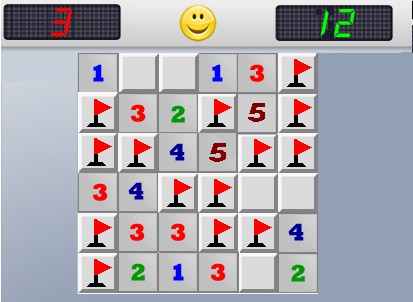
\includegraphics[width=0.35\linewidth]{generado/an-montevideo-oculto.png}
\caption{PNG recuperado de \texttt{montevideo.bmp}}
\label{fig:q4-buscaminas}
\end{figure}

\lstinputlisting[caption={Contenido de \texttt{sol5.txt}},label={lst:q4-sol5}]{generado/an-sol5.txt}

\textbf{Un mensaje en el tablero.} Según \texttt{sol5.txt}, cada mina es un 1, cada fila es una letra y los caracteres ASCII empiezan con \texttt{01}.
Resolviendo las celdas cerradas, las filas dan (cuadro~\ref{tab:q4-tablero}) <<AesOfb>>: el algoritmo es \texttt{aes256} (el de clave de 256 bits) y el modo \texttt{ofb}.

\begin{table}[htbp]
\centering
\small
\begin{tabular}{@{}cccc@{}}
\toprule
Fila & Bits (1 = mina) & Byte & Carácter \\
\midrule
1 & 000001 & \texttt{0x41} & \texttt{A} \\
2 & 100101 & \texttt{0x65} & \texttt{e} \\
3 & 110011 & \texttt{0x73} & \texttt{s} \\
4 & 001111 & \texttt{0x4F} & \texttt{O} \\
5 & 100110 & \texttt{0x66} & \texttt{f} \\
6 & 100010 & \texttt{0x62} & \texttt{b} \\
\bottomrule
\end{tabular}
\caption{Lectura del tablero de buscaminas}
\label{tab:q4-tablero}
\end{table}

\textbf{La contraseña.} El PDF extraído de \texttt{avatar.bmp} con LSBI dice <<La password es metadata>> (listado~\ref{lst:q4-pdf}). Con esos tres datos se
descifra \texttt{secreto1.bmp} (Cuestión~V).

\lstinputlisting[caption={Texto del PDF extraído de \texttt{avatar.bmp}},label={lst:q4-pdf}]{generado/an-avatar-texto.txt}
